\begin{refsection}

\chapter{Introduction}

Fusion energy is the way of the future, and to make the future a reality, the problem of confinement have to be solved. 
In order to produce net energy from fusion, the ion heat energy have to be sufficiently confined that the plasma could be maintained at the necessary high temperature without a need for excessive external heating. This requirement often expressed as the Lawson Triple Product:
\begin{align}
    nT\tau_{E} &\geq 10^{24} [eV m^{-3}s] &\text{  for T $\approx$ 15KeV D-T fusion.}
\end{align}
where n is the density, T is the temperature and $\tau_{E}$ is the energy confinement time of the D-T ions. Of the three values, the confinement time is the one that we have the least direct control over, and involves complex plasma behavior and interactions that needs to be better understood. A significant portion of fusion related plasma physics research involves the understanding, control and design optimization of confinement. A wide variety of confinement strategies area available, broadly separated into magnetic confinement and inertial confinement. Where as the inertial confinement focuses on short, repeated pulses of fusion reaction at very high densities typically driven by enormous lasers, magnetic confinement focus on using the magnetic field to restrict the movement of plasma particles long enough to produce net fusion power. 


\section{Ion confinement in magnetically confined fusion plasmas}

In an ideal world, plasmas would be collisionless, fields would be straight and infinite, there would not be drifts or gradients, and then, there would be no transport. 

The transport mechanisms are usually divided based on which non-ideal factors are introduced back into consideration. With collisions, gradients, and an infinitely repeating cylindrical magnetic geometry, we get classical transport; add toroidicity and the banana orbits that results, we get neo-classical transport; add magnetic wave and turbulence, we get turbulent transport. In addition to these, there is also transport and transport-like processes that don't neatly fall into any category, and then there is the anomalous transport, from processes that we either don't understand, or are not sure of.

\subsection{Classical transport}

Classical transport results from Coulomb collisions of 
Classical transport arises from collisions, and thus the crucial quantity is the collision frequency. To derive it, on has to first consider the fact that sub-atomic particles do not collide like billiard balls, but instead through Coulomb (electro-static) interactions

\subsection{Neo-classical transport}

Neoclassical transport is, to an approximation, due to the toroidal curvature inherent toroidal devices. The inboard side will necessarily have a higher toroidal B field than the outboard side.

\subsection{Turbulence and anomalous transport}

\subsection{Other transport processes}

\section{The reversed field pinch and ion confinement challenges}

\begin{figure}[!htb]
	\centering
	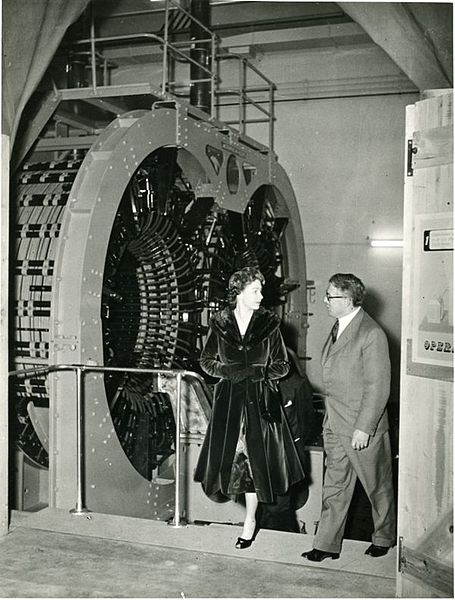
\includegraphics[width = 0.75\linewidth]{./1_Introduction/queen_at_zeta.jpg}
    \label{fig:Queen_at_ZETA}
    \caption[Queen Elizabeth II at the ZETA experiment]{Queen Elizabeth II of Canada visting ZETA during it's construction in 1957. Photograph by UKAEA}
\end{figure}%

The story of the RFP starts with the Zero Energy Thermonuclear Assembly (ZETA). Initially built as an extension of the now abandoned toroidal pinch confinement concept, ZETA was one of the leading fusion experiment of its time. Scientists at ZETA to discover the spontaneous reversal of the magnetic field associated with the most stable (quiescent) period of ZETA's plasmas \cite{Butt_IAEA66,Robinson_IAEA69}. This phenomenon was explained by J. Taylor in 1974 as a naturally result from the relaxation of the magnetic topology towards lower energy state \cite{Taylor74}. These were the foundational documents of the RFP.

\begin{align}\label{eqn:helicity}
	K \equiv \int_{V} \vec{A} \cdot \vec{B} d\tau
\end{align}

Specifically, Taylor posited that in a toroidal plasma of finite resistivity constrained by a perfectly conducting shell, the magnetic helicity $K$ is conserved (eqn. \ref{eqn:helicity}). With this constraint, the plasma relaxes toward a state of minimum magnetic energy characterized by eqn. \ref{eqn:min_energy_condition}, where $\mu \varpropto K/ \Psi ^2$, is a constant unrelated to permeability . 

\begin{align}\label{eqn:min_energy_condition}
    \nabla \times \vec{B} = \mu \vec{B}
\end{align}

In cylindrical approximation, the solution to equation \ref{eqn:min_energy_condition} are Bessel functions (eqn. \ref{eqn:rfp_solution}) where $B_Z$ reverses in the edge if the plasma current is high compared to toroidal flux \cite{Taylor74}.

\begin{align}\label{eqn:rfp_solution}
B_z &= B_0J_0(\mu r)\\
B_\theta &= B_0 J_1(\mu r)\\
B_r & = 0
\end{align}

The magnetic topology of atypical RFP is shown in figure \ref{fig:RFP_geometry}. The relatively low $B_t$ means the RFP have several advantages over the Tokamak. In the tokamaks, powerful toroidal field coils (TF coils) are used to generate toroidal flux and keep the safety factor q is kept above 1 in order to stabilize the plasma. This leads to limits on the toroidal plasma current depending on the the available coil generated toroidal flux. This in turns is limited by engineering constrains in terms of magnetic coil construction. The reversed field pinch avoids these constrains, and
consequently can be constructed with much simpler and cheaper TF coil arrangements, as well as being more easily reach very high current levels to take advantage of large Ohmic heating, possibly to ignition levels.

\begin{figure}[!htb]
	\centering
	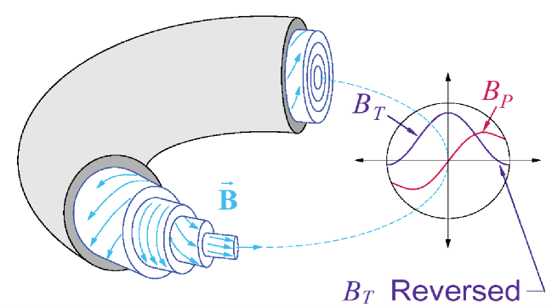
\includegraphics[width = 1.\linewidth]{./1_Introduction/RFP_mag_geometry.png}
	\label{fig:RFP_geometry}
	\caption[RFP magnetic topology]{Illustration of the RFP topology. The most distinct features of the RFP is the similar magnitudes of $B_t$ vs. $B_p$, as well as the fact that $B_p$ reverses direction near the edge.}
\end{figure}%

However, the magnetic topology also poses challenges to the RFP's confinement characteristics. Taylor noted that the relaxation of the magnetic field is made possible by the finite resistivity, but did not speculate on the 'method' of
relaxation. Experiments have shown that the relaxation occurs via resistive tearing mode instabilities which poses a challenge to RFP confinement characteristics.

\begin{figure}
	\centering
    \label{fig:q_profile}
    
    \caption[Example RPF q profile]{q profile typical of the plasmas studies in this work. Note the closely space resonant surfaces.}

\end{figure}

Research into the RFP configuration led to a series of larger and higher current devices. Currently the leading RFP research devices are the Reversed-Field eXperiment\cite{Bartiromo1999RecentExperiment} (RFX) in Padua, Italy, and the Madison Symmetric Torus\cite{Dexter1991} (MST) in Madison, Wisconsin. Comparatively, RFX is capable of driving significantly higher current for a longer duration, where as MST was designed around a close fitting conducting shell to stabilize resistive wall modes.

%TODO: elaborate on RFP ion confinement in standard plasmas, sawtooth, anomalous heating and such.

\section{Improving confinement with inductive current profile control}

PPCD, it's effects, it's characteristics, bursts in PPCD.

\section{What this thesis is about: 1-D classical transport modeling}


As for the structure, I start out with a discussion...
Make no mistake, the interesting parts of this thesis are in chapter \ref{ch:results} and chapter \ref{ch:m0}. However the preceding chapter is an adventure in what went into getting those results and why one should put any weight on them.





\end{refsection}